\begin{frame}
\frametitle{I do not believe in neutrinos}
\begin{columns}
\column{0.35\textwidth}
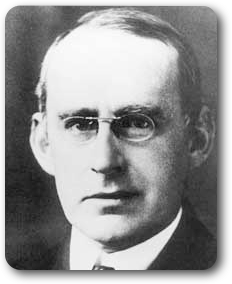
\includegraphics[scale=0.3]{eddington.png}
 
 \column{0.6\textwidth}
%\begin{block}{}
Sir Arthur Eddington: ``Just now nuclear physicists are writing a great deal about hypothetical particles called neutrinos supposed to account for certain peculiar facts observed in $\beta$-ray disintegration. We can perhaps best describe the neutrinos as little bits of spin-energy that have got detached. I am not much impressed by the neutrino theory. In an ordinary way I might say that I do not believe in neutrinos... But I have to reflect that a physicist may be an artist, and you never know where you are with artists. My old-fashioned kind of disbelief in neutrinos is scarcely enough. Dare I say that experimental physicists will not have sufficient ingenuity to make neutrinos?"

%\end{block}
\end{columns}
\end{frame}
